%%%% Preamble:

\documentclass[12pt,a4paper]{article}

\textheight=230mm
\textwidth=160mm
\oddsidemargin=7mm
\evensidemargin=-10mm
\topmargin=-10mm
\headsep=20mm
\columnsep=5mm
\renewcommand{\textfraction}{0.01}
\renewcommand{\floatpagefraction}{0.99}
\renewcommand{\topfraction}{0.9}
\renewcommand{\bottomfraction}{0.9}
\setlength{\hoffset}{-2cm}
\setlength{\voffset}{-2cm}
\topmargin=0.5cm
\oddsidemargin=2.5cm
\textwidth=16cm
\textheight=22cm
\raggedbottom
\sloppy

\usepackage{epsfig}
\usepackage[utf8]{inputenc}
\usepackage{multicol}
\usepackage{authblk}
\usepackage{blindtext}
\usepackage{amssymb}
\usepackage{amsmath}
\usepackage{amsthm}
\usepackage{slashed}
\usepackage{caption}
\usepackage{subcaption}
\usepackage{hyperref}
\usepackage{url}
\usepackage{color}
\usepackage{graphicx}
\usepackage{multirow}
\usepackage{enumerate}
\usepackage{makeidx}
\usepackage{setspace}
\usepackage{lineno}
\usepackage{mciteplus}
\usepackage{cite}
\usepackage{ifthen}
\usepackage{tabularx}
%\include{alias}

\usepackage{xspace}
\usepackage{colortbl}
\usepackage[usenames,dvipsnames]{xcolor}
\usepackage{rotating}
\usepackage{subfig}
\usepackage{lscape}
\usepackage{amsfonts}
\usepackage{upgreek}
\usepackage{units}
%\usepackage[pdftex,
%    plainpages=false,
%    bookmarks         = true,
%    bookmarksnumbered = true,
%    pdfpagemode       = None,
%    pdfstartview      = FitH,
%    pdfpagelayout     = SinglePage,
%    colorlinks        = true,
%    linkcolor         = blue,
%    pagecolor         = black,
%    urlcolor          = blue,
%    pdfborder         = {0 0 0}
%    ]{hyperref}%                             

%\newboolean{articletitles}
%\setboolean{articletitles}{true}
\newboolean{inbibliography}
\setboolean{inbibliography}{false}
%\newboolean{pdflatex}
%\setboolean{pdflatex}{true}
%\newboolean{uprightparticles}
%\setboolean{uprightparticles}{false}

%\usepackage{float}
%\floatstyle{plaintop}
%\restylefloat{table}

\newcommand{\blankpage}{
\newpage
\thispagestyle{empty}
\mbox{}
\newpage
}

\newcommand{\spc}{
\\
\\
}
    
%%%%%%% Main document:
\definecolor{heartgold}{rgb}{0.5, 0.5, 0.0}
\def\gauss      {\mbox{\textsc{Gauss}}\xspace}
\def\photos     {\mbox{\textsc{Photos}}\xspace}
\def\pythia     {\mbox{\textsc{Pythia}}\xspace}
\def\evtgen     {\mbox{\textsc{EvtGen}}\xspace}
\def\geant      {\mbox{\textsc{Geant4}}\xspace}

\def\ptot       {\mbox{$p$}\xspace}
\def\pt         {\mbox{$p_{\rm T}$}\xspace}
\def\et         {\mbox{$E_{\rm T}$}\xspace}


 \def\PA      {\ensuremath{A}\xspace}                 
 \def\PB      {\ensuremath{B}\xspace}                 
 \def\PC      {\ensuremath{C}\xspace}                 
 \def\PD      {\ensuremath{D}\xspace}                 
 \def\PE      {\ensuremath{E}\xspace}                 
 \def\PF      {\ensuremath{F}\xspace}                 
 \def\PG      {\ensuremath{G}\xspace}                 
 \def\PH      {\ensuremath{H}\xspace}                 
 \def\PI      {\ensuremath{I}\xspace}                 
 \def\PJ      {\ensuremath{J}\xspace}                 
 \def\PK      {\ensuremath{K}\xspace}                 
 \def\PL      {\ensuremath{L}\xspace}                 
 \def\PM      {\ensuremath{M}\xspace}                 
 \def\PN      {\ensuremath{N}\xspace}                 
 \def\PO      {\ensuremath{O}\xspace}                 
 \def\PP      {\ensuremath{P}\xspace}                 
 \def\PQ      {\ensuremath{Q}\xspace}                 
 \def\PR      {\ensuremath{R}\xspace}                 
 \def\PS      {\ensuremath{S}\xspace}                 
 \def\PT      {\ensuremath{T}\xspace}                 
 \def\PU      {\ensuremath{U}\xspace}                 
 \def\PV      {\ensuremath{V}\xspace}                 
 \def\PW      {\ensuremath{W}\xspace}                 
 \def\PX      {\ensuremath{X}\xspace}                 
 \def\PY      {\ensuremath{Y}\xspace}                 
 \def\PZ      {\ensuremath{Z}\xspace}                 
 \def\Pa      {\ensuremath{a}\xspace}                 
 \def\Pb      {\ensuremath{b}\xspace}                 
 \def\Pc      {\ensuremath{c}\xspace}                 
 \def\Pd      {\ensuremath{d}\xspace}                 
 \def\Pe      {\ensuremath{e}\xspace}                 
 \def\Pf      {\ensuremath{f}\xspace}                 
 \def\Pg      {\ensuremath{g}\xspace}                 
 \def\Ph      {\ensuremath{h}\xspace}                 
 \def\Pi      {\ensuremath{i}\xspace}                 
 \def\Pj      {\ensuremath{j}\xspace}                 
 \def\Pk      {\ensuremath{k}\xspace}                 
 \def\Pl      {\ensuremath{l}\xspace}                 
 \def\Pm      {\ensuremath{m}\xspace}                 
 \def\Pn      {\ensuremath{n}\xspace}                 
 \def\Po      {\ensuremath{o}\xspace}                 
 \def\Pp      {\ensuremath{p}\xspace}                 
 \def\Pq      {\ensuremath{q}\xspace}                 
 \def\Pr      {\ensuremath{r}\xspace}                 
 \def\Ps      {\ensuremath{s}\xspace}                 
 \def\Pt      {\ensuremath{t}\xspace}                 
 \def\Pu      {\ensuremath{u}\xspace}                 
 \def\Pv      {\ensuremath{v}\xspace}                 
 \def\Pw      {\ensuremath{w}\xspace}                 
 \def\Px      {\ensuremath{x}\xspace}                 
 \def\Py      {\ensuremath{y}\xspace}                 
 \def\Pz      {\ensuremath{z}\xspace}                 

\def\quark     {\ensuremath{\Pq}\xspace}
\def\quarkbar  {\ensuremath{\overline \quark}\xspace}
\def\qqbar     {\ensuremath{\quark\quarkbar}\xspace}
\def\uquark    {\ensuremath{\Pu}\xspace}
\def\uquarkbar {\ensuremath{\overline \uquark}\xspace}
\def\uubar     {\ensuremath{\uquark\uquarkbar}\xspace}
\def\dquark    {\ensuremath{\Pd}\xspace}
\def\dquarkbar {\ensuremath{\overline \dquark}\xspace}
\def\ddbar     {\ensuremath{\dquark\dquarkbar}\xspace}
\def\squark    {\ensuremath{\Ps}\xspace}
\def\squarkbar {\ensuremath{\overline \squark}\xspace}
\def\ssbar     {\ensuremath{\squark\squarkbar}\xspace}
\def\cquark    {\ensuremath{\Pc}\xspace}
\def\cquarkbar {\ensuremath{\overline \cquark}\xspace}
\def\ccbar     {\ensuremath{\cquark\cquarkbar}\xspace}
\def\bquark    {\ensuremath{\Pb}\xspace}
\def\bquarkbar {\ensuremath{\overline \bquark}\xspace}
\def\bbbar     {\ensuremath{\bquark\bquarkbar}\xspace}
\def\tquark    {\ensuremath{\Pt}\xspace}
\def\tquarkbar {\ensuremath{\overline \tquark}\xspace}
\def\ttbar     {\ensuremath{\tquark\tquarkbar}\xspace}


\def\Vud  {\ensuremath{|V_{\uquark\dquark}|}\xspace}
\def\Vcd  {\ensuremath{|V_{\cquark\dquark}|}\xspace}
\def\Vtd  {\ensuremath{|V_{\tquark\dquark}|}\xspace}
\def\Vus  {\ensuremath{|V_{\uquark\squark}|}\xspace}
\def\Vcs  {\ensuremath{|V_{\cquark\squark}|}\xspace}
\def\Vts  {\ensuremath{|V_{\tquark\squark}|}\xspace}
\def\Vub  {\ensuremath{|V_{\uquark\bquark}|}\xspace}
\def\Vcb  {\ensuremath{|V_{\cquark\bquark}|}\xspace}
\def\Vtb  {\ensuremath{|V_{\tquark\bquark}|}\xspace}

% file for definitions that were not available in lhcb-symbols-def.tex

\newcommand{\Af}{\ensuremath{\mathcal{A}_f}\xspace}
\newcommand{\Ak}{\ensuremath{\mathcal{A}_k}\xspace}
\newcommand{\Abarf}{\ensuremath{\bar{\mathcal{A}}_f}\xspace}
\newcommand{\Abark}{\ensuremath{\bar{\mathcal{A}}_k}\xspace}
\newcommand{\Afbar}{\ensuremath{\mathcal{A}_{\bar{f}}}\xspace}
\newcommand{\Akbar}{\ensuremath{\mathcal{A}_{\bar{k}}}\xspace}
\newcommand{\Abarfbar}{\ensuremath{\bar{\mathcal{A}}_{\bar{f}}}\xspace}
\newcommand{\Abarkbar}{\ensuremath{\bar{\mathcal{A}}_{\bar{k}}}\xspace}

\newcommand{\invps}{\ensuremath{ps^{-1}}\xspace}
\newcommand{\rad}{\ensuremath{\rm rad}\xspace}
\def\BuToJPsiK {\decay{\Bu}{\jpsi\Kp}\xspace}
\newcommand{\brackets}[1]{\ensuremath{\left[ #1 \right]}}
\newcommand{\cAbarfbar}{\ensuremath{\bar{\mathcal{A}}_{\bar{f}}}\xspace}
\newcommand{\braket}[2]{\ensuremath{\langle #1|#2\rangle}} % {a}{b}
\newcommand{\cAbarf}{\ensuremath{\bar{\mathcal{A}}_f}\xspace}

\def\cosTmu  {\ensuremath{\cos(\theta_{\mu})}\xspace}

\def\lhcb {\mbox{LHCb}\xspace}
\def\mum  {\ensuremath{\rm \mu m}\xspace}
\def\Jmm {\jpsi(\mumu)}
\def\BsJPsimmPhi {\decay{\Bs}{\jpsi(\mumu)\phi(KK)}\xspace}
\def\BcJPsimunu {\decay{\Bc}{\Jmm \mup \Pnu}}
\newcommand{\CL}{C.L.\ }
\def\CP                {\ensuremath{C\!P}\xspace}
\newcommand{\CLsb}{\ensuremath{\textrm{CL}_{\textrm{s+b}}}\xspace}
\newcommand{\CLs}{\ensuremath{\textrm{CL}_{\textrm{s}}}\xspace}
\newcommand{\CLb}{\ensuremath{\textrm{CL}_{\textrm{b}}}\xspace}
\newcommand{\MC}{Monte Carlo\xspace}

\def\Ppsi {\ensuremath{\psi}\xspace}
\def\jpsi     {{\ensuremath{{\PJ\mskip -3mu/\mskip -2mu\Ppsi\mskip 2mu}}}\xspace}
\def\Jpsi     {{\ensuremath{\jpsi}}\xspace}

\newcommand{\bb}{\ensuremath{b\bar{b}}\xspace}
\newcommand{\mKK}{\ensuremath{m_{KK}}\xspace}
\newcommand{\mkpi}{\ensuremath{m_{\Km\pip}}\xspace}
\newcommand{\mkk}{\mKK}

\newcommand{\bbdim}{\ensuremath{b\bar{b}\to \mu \mu X}\xspace}
\newcommand{\mbdim}{\ensuremath{pp\to \mu \mu X}\xspace}
\newcommand{\Bq}{\ensuremath{B^0_q}\xspace}


\def\Bbar    {\kern 0.18em\overline{\kern -0.18em B}{}\xspace}

\newcommand{\Bs}{\ensuremath{B^0_s}\xspace}
\newcommand{\Bsd}{\ensuremath{B^0_{(s)}}\xspace}
\def\Bsb     {\ensuremath{\Bbar^0_s}\xspace}

\newcommand{\Bd}{\ensuremath{B^0}\xspace}
\def\Bdb     {\ensuremath{\Bbar^0}\xspace}
\newcommand{\Bu}{\ensuremath{B^+}\xspace}
\newcommand{\Bub}{\ensuremath{B^-}\xspace}
\newcommand{\B}{\ensuremath{B}\xspace}
\newcommand{\ket}[1]{\ensuremath{|#1\rangle}}  
\newcommand{\Dst}{\ensuremath{D^{*}}\xspace}
\newcommand{\Dstpm}{\ensuremath{D^{*\pm}}\xspace}
\def\Plambda{\ensuremath{\Lambda}\xspace}
\mathchardef\PLambda="7103
\newcommand{\Lambdab}{\ensuremath{\PLambda^0_b}\xspace}
\newcommand{\Lb}{\Lambdab}
\newcommand{\Lbb}{\Lambdab}
\newcommand{\Bsmumu}{\ensuremath{\Bs\to\mu^+\mu^-}\xspace}
\newcommand{\Jpsimm}{\ensuremath{\Jpsi\to\mu^+\mu^-}\xspace}
\newcommand{\Bdmumu}{\ensuremath{\Bd\to\mu^+\mu^-}\xspace}
\newcommand{\KstKpi}{\ensuremath{\Kst\to K^+\pi^-}\xspace}
\newcommand{\DKpi}{\ensuremath{\D\to K^-\pi^+}\xspace}
\newcommand{\Bsmumugamma}{\ensuremath{\Bs\to\mu^+\mu^-\gamma}\xspace}
\newcommand{\Bdpipi}{\ensuremath{\Bd\to\pi^+\pi^-}\xspace}
\newcommand{\Bspipi}{\ensuremath{\Bs\to\pi^+\pi^-}\xspace}
\newcommand{\BsKK}{\ensuremath{\Bs\to K^+K^-}\xspace}
\newcommand{\BdKK}{\ensuremath{\Bd\to K^+K^-}\xspace}
\newcommand{\BdKpi}{\ensuremath{\Bd\to K^+\pi^-}\xspace}
\newcommand{\BspiK}{\ensuremath{\Bs\to\pi^+K^-}\xspace}
\newcommand{\Bhh}{\ensuremath{B^0_{(s)}\to h^+h^-}\xspace}
\newcommand{\Bmm}{\ensuremath{B^0_{(s)}\to \mu^+\mu^-}\xspace}
\newcommand{\Buhhh}{\ensuremath{B^{\pm}\to h^+h^-h^{\pm}}\xspace}
\newcommand{\BsDspi}{\ensuremath{B^0_{(s)}\to  D^-_s(K^+K^-\pi^-) \pi^+}\xspace}\newcommand{\Kst}{\ensuremath{K^{*0}}\xspace}
\newcommand{\BJpsiX}{\ensuremath{B_{q}\to \jpsi X}\xspace}
\newcommand{\BJpsihh}{\ensuremath{B\to \jpsi h^+h^-}\xspace}
\newcommand{\BuJpsiK}{\ensuremath{B^+\to \jpsi K^+}\xspace}
\newcommand{\BuJpsiKpipi}{\ensuremath{B^\pm\to \jpsi (K\pi\pi)^\pm}\xspace}
\newcommand{\BuJpsimumuK}{\ensuremath{B^+\to \jpsi(\mu^+\mu^-)K^+}\xspace}
\newcommand{\BJpsimumuX}{\ensuremath{B \to \jpsi(\mu^+\mu^-)X}\xspace}
\newcommand{\BdJpsiKst}{\ensuremath{B^0\to \jpsi K^{*0}}\xspace}
\newcommand{\BdJpsiKpi}{\ensuremath{B^0\to \jpsi \Kp \pim}\xspace}
\newcommand{\BJpsiKpi}{\ensuremath{B^0_{(s)}\to \jpsi K \pi}\xspace}
\newcommand{\BsJpsiKpi}{\ensuremath{B^0_s\to \jpsi \Km \pip}\xspace}
\newcommand{\CBsJpsiKst}{\ensuremath{\bar{B^0_s}\to \jpsi \Kst}\xspace}
\newcommand{\BqtoX}{\ensuremath{B_q\to X}\xspace}
\newcommand{\BsJpsiKst}{\ensuremath{B^0_s\to \jpsi \Kstarzb}\xspace}
\newcommand{\BJpsiKst}{\ensuremath{B^0_{(s)}\to \jpsi K^{*0}(\Kstarzb)}\xspace}

\newcommand{\BsKstKst}{\ensuremath{\Bs\to\Kstarz\Kstarzb}\xspace}
\newcommand{\BdJpsimumuKstKpi}{\ensuremath{B^0\to \jpsi(\mu^+\mu^-)K^{*0}(K^+\pi^-)}\xspace}
\newcommand{\BsJpsimumuKstKpi}{\ensuremath{B^0_s\to \jpsi(\mu^+\mu^-)K^{*0}(K^+\pi^-)}\xspace}
\newcommand{\BcJpsimumumunu}{\ensuremath{B^+_c\to \jpsi(\mu^+\mu^-)\mu^+\nu_{\mu}}\xspace}
\newcommand{\Jpsimumu}{\ensuremath{\jpsi\to \mu^+\mu^-}\xspace}

\newcommand{\Bqmumu}{\ensuremath{\ensuremath{B^0_{q}}\to\mu^+\mu^-}\xspace}
\newcommand{\BsJpsimumuPhiKK}{\ensuremath{B^0_s\to \jpsi(\mu^+\mu^-) \phi(K^+K^-)}\xspace}
\newcommand{\BdJpsimumupipi}{\ensuremath{B^0\to \jpsi(\mu^+\mu^-) \pi^+\pi^-}\xspace}
\newcommand{\BdJpsiRho}{\ensuremath{B^0\to \jpsi \rho^0}\xspace}
\newcommand{\BdJpsiRhoI}{\ensuremath{B^0\to \jpsi \rho^0(\pi^+\pi^-)}\xspace}
\newcommand{\BdJpsirho}{\BdJpsiRhoI}
\newcommand{\BdJpsipipi}{\ensuremath{B^0\to \jpsi \pi^+\pi^-}\xspace}
\newcommand{\BsJpsipipi}{\ensuremath{B^0_s\to \jpsi \pi^+\pi^-}\xspace}
\newcommand{\BsJpsifnot}{\ensuremath{B^0_s\to \jpsi f_0(980)}\xspace}
\newcommand{\BsJpsifnotI}{\ensuremath{B^0_s\to \jpsi f_0(980)(\pi^+\pi^-)}\xspace}
\newcommand{\BsJpsifz}{\BsJpsifnotI}
\newcommand{\BsJpsiKK}{\ensuremath{B^0_s\to \jpsi K^+K^-}\xspace}
\newcommand{\BdJpsiKK}{\ensuremath{B^0\to \jpsi K^+K^-}\xspace}
\newcommand{\ropipi}{\ensuremath{\rho^0\to \pi^+\pi^-}\xspace}
\newcommand{\Kspizmm}{\ensuremath{\KS\to\pi^0\mu^+\mu^-}\xspace}
\newcommand{\Klpizmm}{\ensuremath{\KL\to\pi^0\mu^+\mu^-}\xspace}
\newcommand{\Kzpizmm}{\ensuremath{\Kz\to\pi^0\mu^+\mu^-}\xspace}
\newcommand{\KLTpi}{\ensuremath{\KL\to\pi^0\pi^+\pi^-}\xspace}
\newcommand{\KSTpi}{\ensuremath{\KS\to\pi^0\pi^+\pi^-}\xspace}
\newcommand{\KLFm}{\ensuremath{\KL\to\mu^+\mu^-\mu^+\mu^-}\xspace}
\newcommand{\KSFm}{\ensuremath{\KS\to\mu^+\mu^-\mu^+\mu^-}\xspace}
\newcommand{\KFm}{\ensuremath{\Kz\to\mu^+\mu^-\mu^+\mu^-}\xspace}
\newcommand{\KLTmTg}{\ensuremath{\KL\to\mu^+\mu^-\gamma\gamma}\xspace}
\newcommand{\KSTmTg}{\ensuremath{\KS\to\mu^+\mu^-\gamma\gamma}\xspace}
\newcommand{\KTmTg}{\ensuremath{\Kz\to\mu^+\mu^-\gamma\gamma}\xspace}
\newcommand{\KLTg}{\ensuremath{\KL\to\gamma\gamma}\xspace}
\newcommand{\KSTg}{\ensuremath{\KS\to\gamma\gamma}\xspace}

\newcommand{\Kspipi}{\ensuremath{\KS\to\pi^+\pi^-}\xspace}

\newcommand{\Lambdappi}{\ensuremath{\Lambda\to p\pi^-}\xspace}
\newcommand{\Lambdabppi}{\ensuremath{\Lambdab\to p\pi^-}\xspace}
\newcommand{\LambdabpK}{\ensuremath{\Lambdab\to p K^-}\xspace}
\newcommand{\LbJpsipK}{\ensuremath{\Lambdab\to\Jpsi p K^-}\xspace}
\newcommand{\LbJpsippi}{\ensuremath{\Lambdab\to\Jpsi p \pi^-}\xspace}
\newcommand{\LbJpsiph}{\ensuremath{\Lambdab\to\Jpsi p h^-}\xspace}
\newcommand{\BsJpsiPhi}{\ensuremath{B^0_s\to \jpsi \phi}\xspace}
\newcommand{\BsJpsiPhiI}{\ensuremath{B^0_s\to \jpsi \phi(K^+K^-)}\xspace}
\newcommand{\BdJKst}{\BdJpsiKst}
\newcommand{\BuJK}{\BuJpsiK}

\newcommand{\BqJpsiVll}{\ensuremath{B^0_q\to \jpsi V(l^+l^-)}\xspace}
\newcommand{\BqJpsiV}{\ensuremath{B^0_q\to \jpsi V}\xspace}
\newcommand{\Vll}{\ensuremath{V\to l^+ l^-}\xspace}
\newcommand{\BqJpsill}{\ensuremath{B^0_q\to \jpsi l^+l^-}\xspace}

\newcommand{\BsJKst}{\BsJpsiKst}
\newcommand{\BsJphi}{\BsJpsiPhi}
\newcommand{\BsJpsiphi}{\BsJpsiPhiI}
\newcommand{\phis}{\ensuremath{\phi_s}\xspace}
\newcommand{\invfb}{\ensuremath{\text{fb}^{-1}}\xspace}

\def\Kbar  {\kern 0.2em\overline{\kern -0.2em K}{}\xspace}
\def\Kstarzb {\ensuremath{\Kbar^{*0}}\xspace}

\newcommand{\BRof}[1]{\ensuremath{{\cal B}(#1)}\xspace}
\newcommand{\BRvisof}[1]{\ensuremath{{\cal B^{\rm vis}}(#1)}\xspace}
\newcommand{\ps}{\ensuremath{ps}\xspace}
\newcommand{\BR}{\BRof}
\newcommand{\mumu}{\mu\mu}
\newcommand{\pT}{\pt}

\newcommand{\tev}{\ifthenelse{\boolean{inbibliography}}{\ensuremath{~T\kern -0.05em eV}\xspace}{\ensuremath{\mathrm{\,Te\kern -0.1em V}}}\xspace}
\newcommand{\gev}{\ensuremath{\mathrm{\,Ge\kern -0.1em V}}\xspace}
\newcommand{\mev}{\ensuremath{\mathrm{\,Me\kern -0.1em V}}\xspace}
\newcommand{\kev}{\ensuremath{\mathrm{\,ke\kern -0.1em V}}\xspace}
\newcommand{\ev}{\ensuremath{\mathrm{\,e\kern -0.1em V}}\xspace}
\newcommand{\gevc}{\ensuremath{{\mathrm{\,Ge\kern -0.1em V\!/}c}}\xspace}
\newcommand{\mevc}{\ensuremath{{\mathrm{\,Me\kern -0.1em V\!/}c}}\xspace}
\newcommand{\gevcc}{\ensuremath{{\mathrm{\,Ge\kern -0.1em V\!/}c^2}}\xspace}
\newcommand{\gevgevcccc}{\ensuremath{{\mathrm{\,Ge\kern -0.1em V^2\!/}c^4}}\xspace}
\newcommand{\mevcc}{\ensuremath{{\mathrm{\,Me\kern -0.1em V\!/}c^2}}\xspace}

\newcommand{\MeV}{\mev}
\newcommand{\GeV}{\gev}
\newcommand{\TeV}{\tev}
\newcommand{\MeVc}{\mevc}
\newcommand{\GeVc}{\gevc}
\newcommand{\MeVcc}{\mevcc}
\newcommand{\GeVcc}{\gevcc}
\newcommand{\Km}{\ensuremath{K^-}\xspace}
\newcommand{\Kp}{\ensuremath{K^+}\xspace}
\newcommand{\KS  }{\ensuremath{K^0_{\mathrm{\scriptscriptstyle S}}}\xspace} 
\newcommand{\KL  }{\ensuremath{K^0_{\mathrm{\scriptscriptstyle L}}}\xspace} 
\newcommand{\Kz  }{\ensuremath{K^0\xspace} }

\newcommand{\pim}{\ensuremath{\pi^-}\xspace}
\newcommand{\pip}{\ensuremath{\pi^+}\xspace}
\newcommand{\piz}{\ensuremath{\pi^0}\xspace}
\newcommand{\Kstarz}{\Kst}
\newcommand{\invpb}{\ensuremath{\,{\rm pb}^{-1}}\xspace}
\newcommand{\invnb}{\ensuremath{\,{\rm nb}^{-1}}\xspace}
\newcommand{\mb}{\ensuremath{\,{\rm mb}}\xspace}
\newcommand{\microb}{\ensuremath{\,{\rm \mu b}}\xspace}

\newcommand{\Enow}{\ensuremath{\,{\sqrt{s}=7\TeV}}\xspace}
\newcommand{\Einj}{\ensuremath{\,{\sqrt{s}=900\GeV}}\xspace}
\newcommand{\Enom}{\ensuremath{\,{\sqrt{s}=14\TeV}}\xspace}
\newcommand{\Efive}{\ensuremath{\,{\sqrt{s}=10\TeV}}\xspace}
\newcommand{\pdf}{\ensuremath{{\rm PDF}}\xspace}
\newcommand{\pdfs}{\ensuremath{{\rm PDFs}}\xspace}
\newcommand{\IP}{\ensuremath{{\rm IP}}\xspace}
\newcommand{\ThetaK}{\ensuremath{{\Theta_{K^{*}}}}\xspace}
\newcommand{\fdfs}{\ensuremath{\frac{f_d}{f_s}}\xspace}

\newcommand{\DLL}{\ensuremath{{\rm \Delta LL}}\xspace}
\newcommand{\gl}{\ensuremath{{\rm GL}}\xspace}
\newcommand{\glk}{\ensuremath{{\rm GL_K}}\xspace}
\newcommand{\glksm}{\ensuremath{{\rm GL_{KS}}}\xspace}
\newcommand{\glsm}{\ensuremath{{\rm GL_{S}}}\xspace}
\newcommand{\PID}{\ensuremath{{\rm PID}}\xspace}
\newcommand{\etos}{\ensuremath{\epsilon^{TOS/SEL}}\xspace}
\newcommand{\etis}{\ensuremath{\epsilon^{TIS/SEL}}\xspace}
\newcommand{\etistos}{\ensuremath{\epsilon^{TIS\&TOS/SEL}}\xspace}

\newcommand{\etrig}{\ensuremath{\epsilon^{TRIG/SEL}}\xspace}
\newcommand{\eSelect}{\ensuremath{\epsilon^{SEL/REC}}\xspace}
\newcommand{\eReco}{\ensuremath{\epsilon^{REC}}\xspace}

\newcommand{\sumpt}{\ensuremath{{\Sigma \pt}}\xspace}
\newcommand{\maxpt}{\ensuremath{{\rm max_{\pt}}}\xspace}
\newcommand{\maxip}{\ensuremath{\rm max_{\IP}}\xspace}

\newcommand{\swave}{{\rm S--wave}\xspace}
\newcommand{\pwave}{{\rm P--wave}\xspace}
\newcommand{\dwave}{{\rm D--wave}\xspace}
\newcommand{\hwave}{{\rm H--wave}\xspace}
\newcommand{\fwave}{{\rm F--wave}\xspace}

\newcommand{\dAda}{\ensuremath{\frac{ \partial A}{ \partial a}}}
\newcommand{\dAdtheta}{\ensuremath{\frac{\partial A}{\partial \theta}}}
\newcommand{\dHdtheta}{\ensuremath{\frac{\partial H}{\partial \theta}}}
\newcommand{\dHda}{\ensuremath{\frac{\partial H}{\partial a}}}
\newcommand{\dPHIda}{\ensuremath{\frac{\partial \tan\Delta\phi}{\partial a}}}
\newcommand{\dPHIdtheta}{\ensuremath{\frac{\partial \tan\Delta\phi}{\partial \theta}}}


%%%%%%%%%%%%%%%%%%%%%%%%%% Ks->pi0mumu %%%%%%%%%%%%%%%%%%%%%%%%%%%%%%%%%%%
\newcommand\bbone{\ensuremath{\mathds{1}}}
\newcommand{\Mpzmumu}{\ensuremath{M_{\Pgpz\APmuon\Pmuon}}}
\newcommand{\mybox}[2]{{\color{#1}\fbox{\normalcolor#2}}}
\newcommand{\PKzS}{\ensuremath{K^{0}_{S}}}
\newcommand{\PKzL}{\ensuremath{K^{0}_{L}}}
\newcommand{\PKz}{\ensuremath{K^{0}}}
\newcommand{\Plepton}{\text{\it{l}}}
\newcommand{\Pmuon}{\ensuremath{\mu^{-}}}
\newcommand{\APmuon}{\ensuremath{\mu^{+}}}
\newcommand{\Pgpz}{\ensuremath{\pi^{0}}}
\newcommand{\Pgpp}{\ensuremath{\pi^{+}}}
\newcommand{\Pgpm}{\ensuremath{\pi^{-}}}
\newcommand{\Pqd}{\text{\it{d}}}
\newcommand{\Pqs}{\text{\it{s}}}
%\newcommand{\PZ}{\ensuremath{Z^{0}}}
\newcommand{\PBds}{\ensuremath{B^{0}_{d,s}}}
\newcommand{\Pgamma}{\ensuremath{\gamma}}
\newcommand{\KzPzMuMu}{\ensuremath{\Kz\rightarrow\Pgpz\APmuon\Pmuon}}
\newcommand{\KsPzMuMu}{\ensuremath{\KS\rightarrow\Pgpz\APmuon\Pmuon}}
%%%%%%%%%%%%%%%%%%%%%%%%%%%%%%%%%%%%%%%%%%%%%%%%%%%%%%%%%%%%%%%%%%%%%%%%%%



%% These commands can be placed in the preamble (to be a global definition)
%% or locally inside the \begin{table}...\end{table} syntax.
%https://www.msu.edu/~harris41/latex_tablespacing.html
\newcommand\Tstrut{\rule{0pt}{2.6ex}}
\newcommand\TTstrut{\rule{0pt}{3.2ex}}
\newcommand\Bstrut{\rule[-1.2ex]{0pt}{0pt}}
\newcommand\BBstrut{\rule[-1.8ex]{0pt}{0pt}}
\newcommand{\rhoJ}{\ensuremath{\rho_{\Jpsi}}\xspace}
\newcommand{\equref}[1]{Eq.~\ref{#1}}
\newcommand{\figref}[1]{Fig.~\ref{#1}}
\newcommand{\tabref}[1]{Table~\ref{#1}}
\newcommand{\appref}[1]{Appendix~\ref{#1}}
\newcommand{\bibref}[1]{Ref.~\cite{#1}}
\newcommand{\secref}[1]{Sect.~\ref{#1}}
\newcommand{\cAf}{\ensuremath{\mathcal{A}_f}\xspace}
\newcommand{\cAfbar}{\ensuremath{\mathcal{A}_{\bar{f}}}\xspace}

\newcommand{\tred}[1]{\textcolor{red}{#1}}

\newcommand{\tabcaption}[1]{  %  for tables, so that the caption when above the float is placed correctly
\vspace{-\abovecaptionskip} % 
\caption[#1]{#1}
\vspace{\abovecaptionskip}
}




%%%%%%%%%%%%%%%%%%%%%%%%%%%%%%%%%%%
%
% Symbol definitions for JPsiPhi
%
%%%%%%%%%%%%%%%%%%%%%%%%%%%%%%%%%%%

%\def\bJpsiPhi{B_s \to J/\psi \phi}
%\def\bbarJpsiPhi{\bar{B}_s \to J/\psi \phi}

% particles
\def\bl{B_{\text L}}
\def\bh{B_{\text H}}

\def\BsJKK{$\Bs\to\Jpsi K^+K^-$}

%strong phases
\def\delone{\delta_1}
\def\deltwo{\delta_2}
\def\delpar{\delta_\parallel}
\def\delperp{\delta_\perp}
\def\delzero{\delta_0}
\def\dels{\delta_{\rm S}}
\def\delsperp{\dels - \delperp}

% D-wave
\def\deltwozero{\delta_{20}}
\def\deltwopa{\delta_{2\parallel}}
\def\deltwope{\delta_{2\perp}}

% amplitudes
\def\apar{A_{\|}}
\def\aperp{A_{\perp}}
\def\aparsq{|A_{\|}|^2}
\def\aperpsq{|A_{\perp}|^2}
\def\assq{|A_{s}|^2}
\def\azero{A_{0}(t)}
\def\azerosq{|A_{0}|^2}

% D-wave
\def\atwopa{A_{2\|}}
\def\atwope{A_{2\perp}}
\def\atwozero{A_{2\|}}

\def\aparsqo{|A_{\|}(0)|^2}
\def\aperpsqo{|A_{\perp}(0)|^2}
\def\assqo{|A_{s}(0)|^2}
\def\azerosqo{|A_{0}(0)|^2}

\def\fS{F_{\text{S}}}
\def\maglambda{|\lambda|}


%CP asymmetries
\newcommand{\CP}{\ensuremath{{C\!P}}\xspace}

\newcommand{\ACPL}{\ensuremath{A^{C\!P}_0}\xspace}
\newcommand{\ACPpa}{\ensuremath{A^{C\!P}_{\|}}\xspace}
\newcommand{\ACPpe}{\ensuremath{A^{C\!P}_{\perp}}\xspace}
\newcommand{\ACPS}{\ensuremath{A^{C\!P}_S}\xspace}

%fractions
\newcommand{\fL}{\ensuremath{f_0}\xspace}
\newcommand{\fpa}{\ensuremath{f_{\|}}\xspace}
\newcommand{\fpe}{\ensuremath{f_{\perp}}\xspace}

%Swave parameters in mKpi bins
\newcommand{\AsBinZero}{\ensuremath{F_S\_826\_861}\xspace}
\newcommand{\AsBinOne}{\ensuremath{F_S\_861\_896}\xspace}
\newcommand{\AsBinTwo}{\ensuremath{F_S\_896\_931}\xspace}
\newcommand{\AsBinThree}{\ensuremath{F_S\_931\_966}\xspace}

\newcommand{\dsBinZero}{\ensuremath{\delta_S\_826\_861}\xspace}
\newcommand{\dsBinOne}{\ensuremath{\delta_S\_861\_896}\xspace}
\newcommand{\dsBinTwo}{\ensuremath{\delta_S\_896\_931}\xspace}
\newcommand{\dsBinThree}{\ensuremath{\delta_S\_931\_966}\xspace}

%decay angles
\def\thetatr{\theta_{tr}}
\def\phitr{\phi_{tr}}
\def\psitr{\psi_{tr}}
\def\thetaone{\theta_{\phi}}
\def\thetatwo{\theta_2}

% helicity angles
\def\thetamu{\ensuremath{\theta_{\mu}}\xspace}
\def\thetaK{\ensuremath{\theta_{K}}\xspace}
\def\phihel{\ensuremath{\varphi_{h}}\xspace}


% background model
\def\alphab{\alpha_{\text{bkg}}}


% tagging & resolution
\def\tagomega{\eta}
\def\wtrue{\omega}
\def\wtruebar{\bar\omega}
\def\effmistag{\sqrt{\varepsilon_{tag}} (1 - 2 w) }
\def\eventres{\sigma_t}
\def\eventresscale{r_t}


% For PDF description
\def\LLF{{\cal L}}
\def\fullpdf{{\cal P}}
\def\sigpdf{{\cal S}}
\def\bkgpdf{{\cal B}}
\def\fsig{f_{s}}

% sPlot and sWeights
\newcommand{\splots}   {\mbox{$_s{\cal P}lots$}\xspace}
\newcommand{\splot}    {\mbox{$_s{\cal P}lot$}\xspace}
\newcommand{\sweights} {\mbox{$_s{\cal W}eights$}\xspace}
\newcommand{\sweight}  {\mbox{$_s{\cal W}eight$}\xspace}



\makeindex
\begin{document}

\thispagestyle{empty}

\vspace{3cm}

\begin{center}
{\bf\normalsize UNIVERSIDADE DE SANTIAGO DE COMPOSTELA}
\end{center}
\vspace{0.10cm}
\begin{center}
\normalsize Departamento de F\'isica de Part\'iculas
\end{center}

\vspace{1.5cm}

{\bf\LARGE\boldmath
\begin{center}
New physics implications and searches at LHCb
\end{center}}
%%%%%%%%%%%%%%%%%%%%%%%%%%%
%\vspace{0.25cm}
\vspace{0.5cm}
\begin{center}
%\large\bf{Miriam Lucio Mart\'inez}\\%$^1$}\\
\Large{Miriam Lucio Mart\'inez}\\%$^1$}\\
%\vspace*{0.5cm}
%{\it  $^1$Universidade de Santiago de Compostela, Spain}\\
%%\vspace{0.5cm}
%%\bf{30 de setembro de 2017}
\end{center}
%%%%%%%%%%%%%%%%%%%%%%%%%%%

\vspace{5cm}
\begin{center}
\bf{\LARGE Tese de Doutoramento}\\
\end{center}
\vspace{0.2cm}
\begin{center}

\includegraphics[width=0.35\textwidth]{figs/logo_ux.jpg}
\end{center}
\begin{center}
\vspace{0.2cm}
{\large \bf Programa de Doutoramento}\\\vspace{0.1cm}
{\large \bf en Física Nuclear e de Partículas}
\end{center}

\blankpage
\input{chapters/Signatures}
\blankpage
\input{chapters/Acknowledgements} %
\blankpage
\input{chapters/Abstract} %

\pagenumbering{roman}
\cleardoublepage
\tableofcontents

%%%%% Main chapters

\blankpage
\linenumbers
%\chapter{Introduction}
\label{sec:introduction}
The Standard Model (hereafter SM) of Particle Physics, mainly formulated in the \textcolor{red}{1970s}, is the quantum field theory that describes the strong and electroweak interactions. It is represented in Group Theory by~\cite{PDG}:
\begin{equation}
SU(3)_C\bigotimes SU(2)_T \bigotimes U(1)_Y
\end{equation}
Where the strong interaction, described by Quantum Chromodynamics (QCD), is contained in the $\rm SU(3)_C$ group (a symmetry group of \textit{color}, C), and $SU(2)_T \bigotimes U(1)_Y$, where T and Y stand for weak isospin and hypercharge respectively, relates to the electroweak interaction (EW). 
The SM fermions (described in \ref{subsec:Particles}) consist of three families with two $SU(2)_L$ doublets ($Q_L$ and $L_L$) and three $SU(2)_L$ singlets ($U_R$, $D_R$ and $E_R$). %% MFV_TOTAL
In order to preserve the electroweak gauge invariance (and so, keep the SM renormalizable), the particles predicted by this lagrangian have to be massless. This leads to the necessity of a spontaneously breaking of the symmetry into $SU(3)_C \bigotimes U(1)_{EM}$. Such breaking is done by the vacuum expectation value (VEV) of a scalar isospin doublet, with hypercharge 1/2, called \textit{Higgs}~\cite{Higgs}. More details on this mechanism are given in ~\ref{subsec:Higgs}.
\begin{equation}
G_{SM} \xrightarrow{Higgs(1,2)_{1/2}} SU(3)_C \bigotimes U(1)_{EM}
\end{equation}

\section{Higgs Mechanism}
\label{subsec:Higgs}
Similarly to what happens in the Ginzburg-Landau theory for superconductivity, the Higgs mechanism arises from the need of EWSB, together with the requirement that gauge invariance is preserved in $\mathcal{L}_{SM}$. The Higgs field interacts with the particles corresponding to the elementary field, including gauge bosons. Resulting of this interaction, these particless acquire mass. 
As for the others, the Higgs field has associated at least one particle in the SM, the Higgs boson, a scalar particle with spin zero. Within the SM, it is not possible to make a prediction of its mass (other than setting loose upper and lower limits), since it depends on a parameter that needs to be determined experimentally. 

%%% Higgs term in the lagrangian
The term in the SM lagrangian that accounts for the self-interaction of the Higgs field is the following:
\begin{equation}
\mathcal{L}_{Higgs} = \mu^2\phi^{\dagger} \phi - \lambda (\phi^{\dagger} \phi)^2, \ \mu^2 < 0, \lambda > 0
\end{equation}
Where $\phi$ denotes the (complex) Higgs Field :
\begin{equation}
\phi = \binom{\phi^+}{\phi^0}
\end{equation}
A scalar isospin doublet with hypercharge +1/2. The initial symmetry of the system is broken for a non-zero value of this field:
\begin{equation}
\phi = \frac{1}{\sqrt{2}}\binom{0}{v}, v = \frac{\mu}{\sqrt{\lambda}}
\end{equation}
Leading to the Higgs particle, with mass $\sqrt{2\lambda v^2}$, neutral charge and hypercharge 1. It was discovered in 2012 by 2 detectors at LHC, ATLAS~\cite{ATLASHiggs} and CMS~\cite{CMSHiggs}. Its mass was measured to be $125.09 \pm 0.24 \GeV$.

\begin{figure} [htb!]
\begin{center}
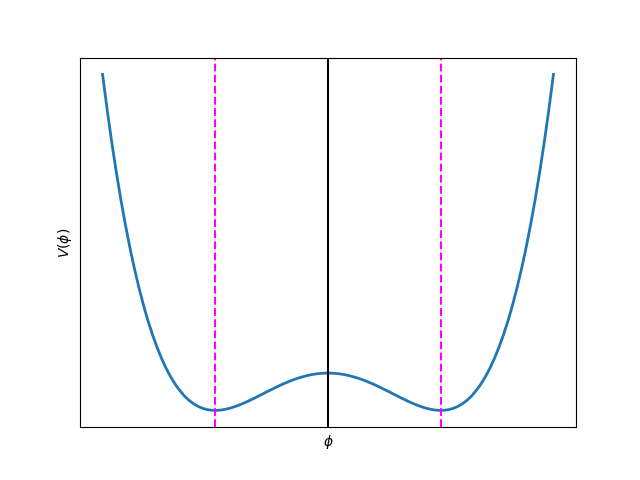
\includegraphics[scale=0.7]{figs/higgs.png}
\caption{Higgs mechanism. The dashed-magenta vertical line indicate the two vacuum states. The black vertical line is located at the origin. The minimum is not at 0, and therefore the potential has a VEV. \label{fig:higgs}}
\end{center}
\end{figure}

The gauge fields $W^\pm$ and Z acquire mass through their interaction with the Higgs boson. Thus:
\begin{equation}
W^\pm = \frac{1}{\sqrt{2}}(W^{(1)} \mp W^{(2)}), \ Z = \frac{1}{\sqrt{g_I^2 + g_Y^2}}(g_IW^{(3)} - g_Y B)
\end{equation}
Where Z and $W^\pm$ are linear combinations of the weak and hypercharge bosons (3 and 1, respectively). Then:
\begin{equation}
m_{W^\pm} = \frac{vg_I}{\sqrt{2}}, m_{Z} = v \sqrt{\frac{g_I^2 + g_Y^2}{2}}
\end{equation}
Notice that the relation between both masses is given by the so-called \textit{weak-mixing angle}, $\theta_W$
\begin{equation}
\frac{m_W^{\pm}}{m_Z} = \frac{g_I}{\sqrt(g_I + g_Y)} = \cos{\theta_W}
\end{equation}
Measured experimentally to be $\theta_W \sim 0.50 \ \rm rad$~\cite{PDG}. 

\subsection{Coupling to fermions}
The lagrangian term corresponding to the Higgs (\textit{H})-fermions (\textit{f}) interaction can be written as follows:
\begin{equation}
\mathcal{L_{Hf}} = - \lambda_e \bar{E}_L \phi E_R - \lambda_d \bar{Q}_L \phi D_{R} - \lambda_u \varepsilon^{ab} \phi_b^{\dagger}U_R + \rm h.c.
\end{equation}
Where $\lambda_e, \lambda_d$ and $\lambda_u$ are the respective coupling constants (\textit{Yukawa couplings}), different for each fermion. Substituting in this expression the Higgs field with the result obtained before:
\begin{equation}
m_e = \frac{v\lambda_e}{\sqrt{2}}, \ m_u = \frac{v\lambda_u}{\sqrt{2}}, \ m_d = \frac{v\lambda_d}{\sqrt{2}}
\end{equation}
The fermion masses are therefore proportional to the Yukawa couplings.

%%% CKM: leptonic case: interaction independent, for each flavor; not quarks
\subsection{Coupling to photons and gluons}
Both gluons and photons are gauge bosons of the strong and electromagnetic interactions, respectively. They have zero mass and spin 1. For the gluons, given that the color symmetry SU(3) is not modified by the Higgs mechanism, they don't directly interact with the Higgs boson. The only way this interaction can happen is via quark loops. 
Contrary to what happens with the gluons, the photons can interact directly with the Higgs field. Nevertheless, they don't acquire mass as a result of this interaction, $m_\gamma = 0$.  

\section{Particle Content}
\label{subsec:Particles}
%% Fermion generatio, representation in the SM gauge symmetry 
The particle content of the SM is categorized as a function of the intrinsic angular momentum of each particle, or \textit{spin}. Particles with half-integer spin are called \textit{fermions}, while those with an integer value for the spin are \textit{bosons}. The latter ones are the carriers of the different interactions that enter the SM lagrangian:
\begin{equation}
\mathcal{L} = \mathcal{L}_{kin} + \mathcal{L}_{Higgs} + \mathcal{L}_{Yuk}
\end{equation}
Where the first term accounts for the kinetic part of the interaction, and the two others describe the Higgs mechanism (described in \ref{subsec:Higgs}) and its interaction with the fermions. 
%\red{W rises when introducing the covariant derivative and explain coupling constants}
Regarding the fermions, a further classification can be made depending on whether they are affected (\textit{quarks}) or not (\textit{leptons}) by the strong interaction. If affected, a quantum number, color, further characterizes the particle. Note that the electroweak interaction affects all the particles. 

An additional quantum number, \textit{flavour}, is used to label the different elementary particles. There are three flavour families of quarks and leptons in the SM, represented in \ref{fig:particle_content}. Each lepton (electron, \textit{i}, muon, $\mu$, tauon, $\tau$) has associated a neutral particle,  called the \textit{neutrino}: $\nu_e$, $\nu_\mu$, $\nu_tau$. Even though they are predicted to be massless within the SM (so that there are not right-handed neutrinos in the SM and, equivalently, there are not left-handed antineutrinos), they are known to have mass~\cite{SolarNeutrinos}.

The elementary particles of the SM are represented in \ref{fig:particle_content}. For each of this particles, there exists another one with the same mass but opposite physical charges. Those are called \textit{antiparticles}. Notice that some particles (e.g. the photon) are their own antiparticle. 

\begin{figure} [htb!]
\begin{center}
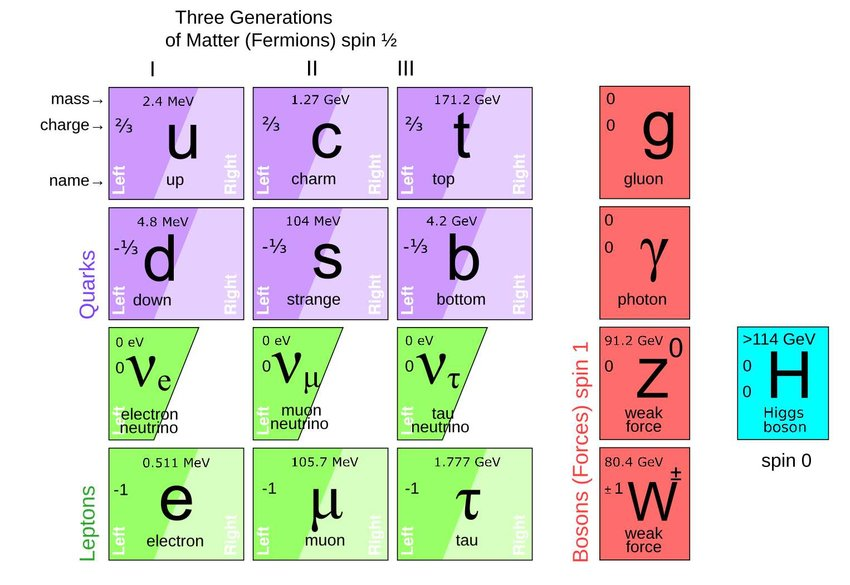
\includegraphics[scale=0.5]{figs/particle_content.jpg}
\caption{The SM particle content\red{~\cite{ParticleContent}}. \label{fig:particle_content}}
\end{center}
\end{figure}

Quarks form bound states named \textit{hadrons} that have a quantum number associated called the baryonic number, $\mathcal{B}$. They are composed either by a quark and an antiquark (forming \textit{mesons}, with $\mathcal{B} = 0$) or by three quarks (\textit{baryons}, with $\mathcal{B}=1$). Given the spin that results of the \textit{sum} of the quarks, baryons are fermions and mesons are bosons. 

\section{CKM Matrix}
\label{sec:CKMMatrix} 
The Yukawa couplings, seen in \ref{subsec:Higgs}, generate off-diagonal terms that allow for the quarks to \textit{mix} between the three generations. Diagonalizing the quark mass matrices, 4 unitary matrices are obtained, $V_{L,R}^{u,d}$, that determine the coupling of the $W^{\pm}$ bosons to the different quarks. 

This diagonalization can be seen as the rotation from one basis ($q$) to another, hereafter called \textit{mass basis} or \textit{physical basis}, $q'$. These are related by the aforementioned matrices ~\cite{CKM}:

\begin{equation}
u_L^i = V_u^{ij} u'^{j}_L \ \ d_L^i = V_d^{ij}d'^{j}_L 
\end{equation}

With this, the weak current transforms from $\bar{u}^i_L \gamma^{\mu} d_L^i$ to $\bar{u}'^i_L \gamma^{\mu}(V_u^{\dag}V_d)_{ij}) d'^i_L \equiv \bar{u}'^i_L \gamma^{\mu} V_{\rm CKM} d'^i_L$, where $V_{\rm CKM}$ is a non-diagonal, unitary matrix called the \textit{Cabibbo-Kobayashi-Maskawa} (CKM) matrix. The most up-to-date measured values of its elements can be found in~\cite{PDG}. 

\begin{equation}
V^{\rm CKM} = \begin{pmatrix}
V_{ud} & V_{us} & V_{ub}\\ 
V_{cd} & V_{cs} & V_{cb}\\ 
V_{td} & V_{ts} & V_{tb}
\end{pmatrix}
\end{equation}

This matrix is the responsible for the transitions between different quark generations, that allow for processes in which there is change in the quark flavour but not in the electric charge to happen. These are known as Flavour Changing Neutral Currents (FCNC). Most of the rare decays are of this type. It also causes CP violation, that will be discussed in the following sections. It is worth noticing that this matrix is not necessarily restricted to being 3x3, thus extra quark generations (not discovered yet) can exist~\cite{CKM}.

%\red{unitarity triangle}\red{... In QCD, flavour is a global symmetry, broken in the electroweak symmetry... }
 
%Yukawa couplings led to off-diagonal elements in the 3x3 matrix between the different families. Diagonalizing the Yukawa matrix (mass matrix), off diagonal elements appear in the charged current coupling (Q+-)
%When the three fermion generations are added to the theory, additional terms mixing quarks of different
%generations are possible. Alternatively, it is possible to diagonalise the Higgs couplings by switching
%to a different basis for the quark fields. Writing the Lagrangian in this alternative basis (hereinafter
%referred to as “mass basis” or “physical basis”) will of course simplify L Y uk but with the cost of causing
%a complication in the gauge side. Calling q the interaction eigenstates and q the mass eigenstates, both
%bases are related through the unitary relations:

\section{Need for New Physics}
%%% Introduction
Even though the SM has shown to be a very successful theory, it lacks explanation for several phenomena present in nature. 

\subsection{Matter-antimatter imbalance}
In order to have an excess of matter over antimatter in the early universe (process known as \textit{baryogenesis}~\cite{Baryogenesis}, three requirements have to be fulfilled. These are known as the \textit{Sakharov conditions}~\cite{Baryogenesis}, and include a large CP-violation. The SM predicts a rate of the CP-violation smaller than the one needed, thus, a new source is required.
%%%%%%%%%%%%%%%%%%%%%%%%%%%%%%%%%%%%%%%%%%%%%%%%%%%%%%%%%%%%%%%%%%%%%%%%%%%%%%%%%%%%%
\subsection{Dark matter and dark energy}
\label{subsec:DarkMatter_DarkEnergy}
Several experimental evidences, such as the rotational speed of spiral galaxies, gravitational lensing, or observed fluctuations in the Cosmic Microwave Background radiation (\red{see for example~\cite{DM1},~\cite{DM2}}) have lead to  discovery of dark matter and dark energy, that take up the vast majority of the Universe composition {and don't interact with light}. The possible baryonic (MACHOs, MAssive Compact Halo Objects, such as black holes, and RAMBOs, Robust Association of Massive Baryonic Objects) percentage of dark matter is small. The rest cannot be explained within the SM, it is \textit{non baryonic cold dark matter}, where cold refers to its non-relativistic nature, \red{or neutrinos}. Possible candidates for cold dark matter entail weakly interacting sub-eV particles (WISPs), such as axions(~\cite{Axions1},~\cite{Axions2},~\cite{Axions3}), primordial back holes \red{ref} and weakly interacting massive particles (WIMPs). 
%%% Experimental signatures

\subsection{Unification of forces}
The behavior of the three coupling constants at the order of TeV,\red{\textit{naturalness}}
,(figure\ref{fig:constants}, left) suggests the existence of a \textit{primary} interaction, represented by a higher symmetry group (e.g. SU(5) or SO(10)). Spontaneous symmetry breaking of this interaction would lead to the existence of the electromagnetic, weak, and strong interactions at lower energy scales. Nevertheless, in order for this to happen, there should be a matching of these coupling constants for such high energies, which is not perfectly achieved in the SM. This hints the existence of new symmetries orfields (figure\ref{fig:constants}, right). Some of these suggestions will be discussed in the following chapter. 

%% IMG source http://www.theo-physik.uni-kiel.de/~bonitz/public/nobel04/public.html
\begin{figure} [htb!]
\begin{center}
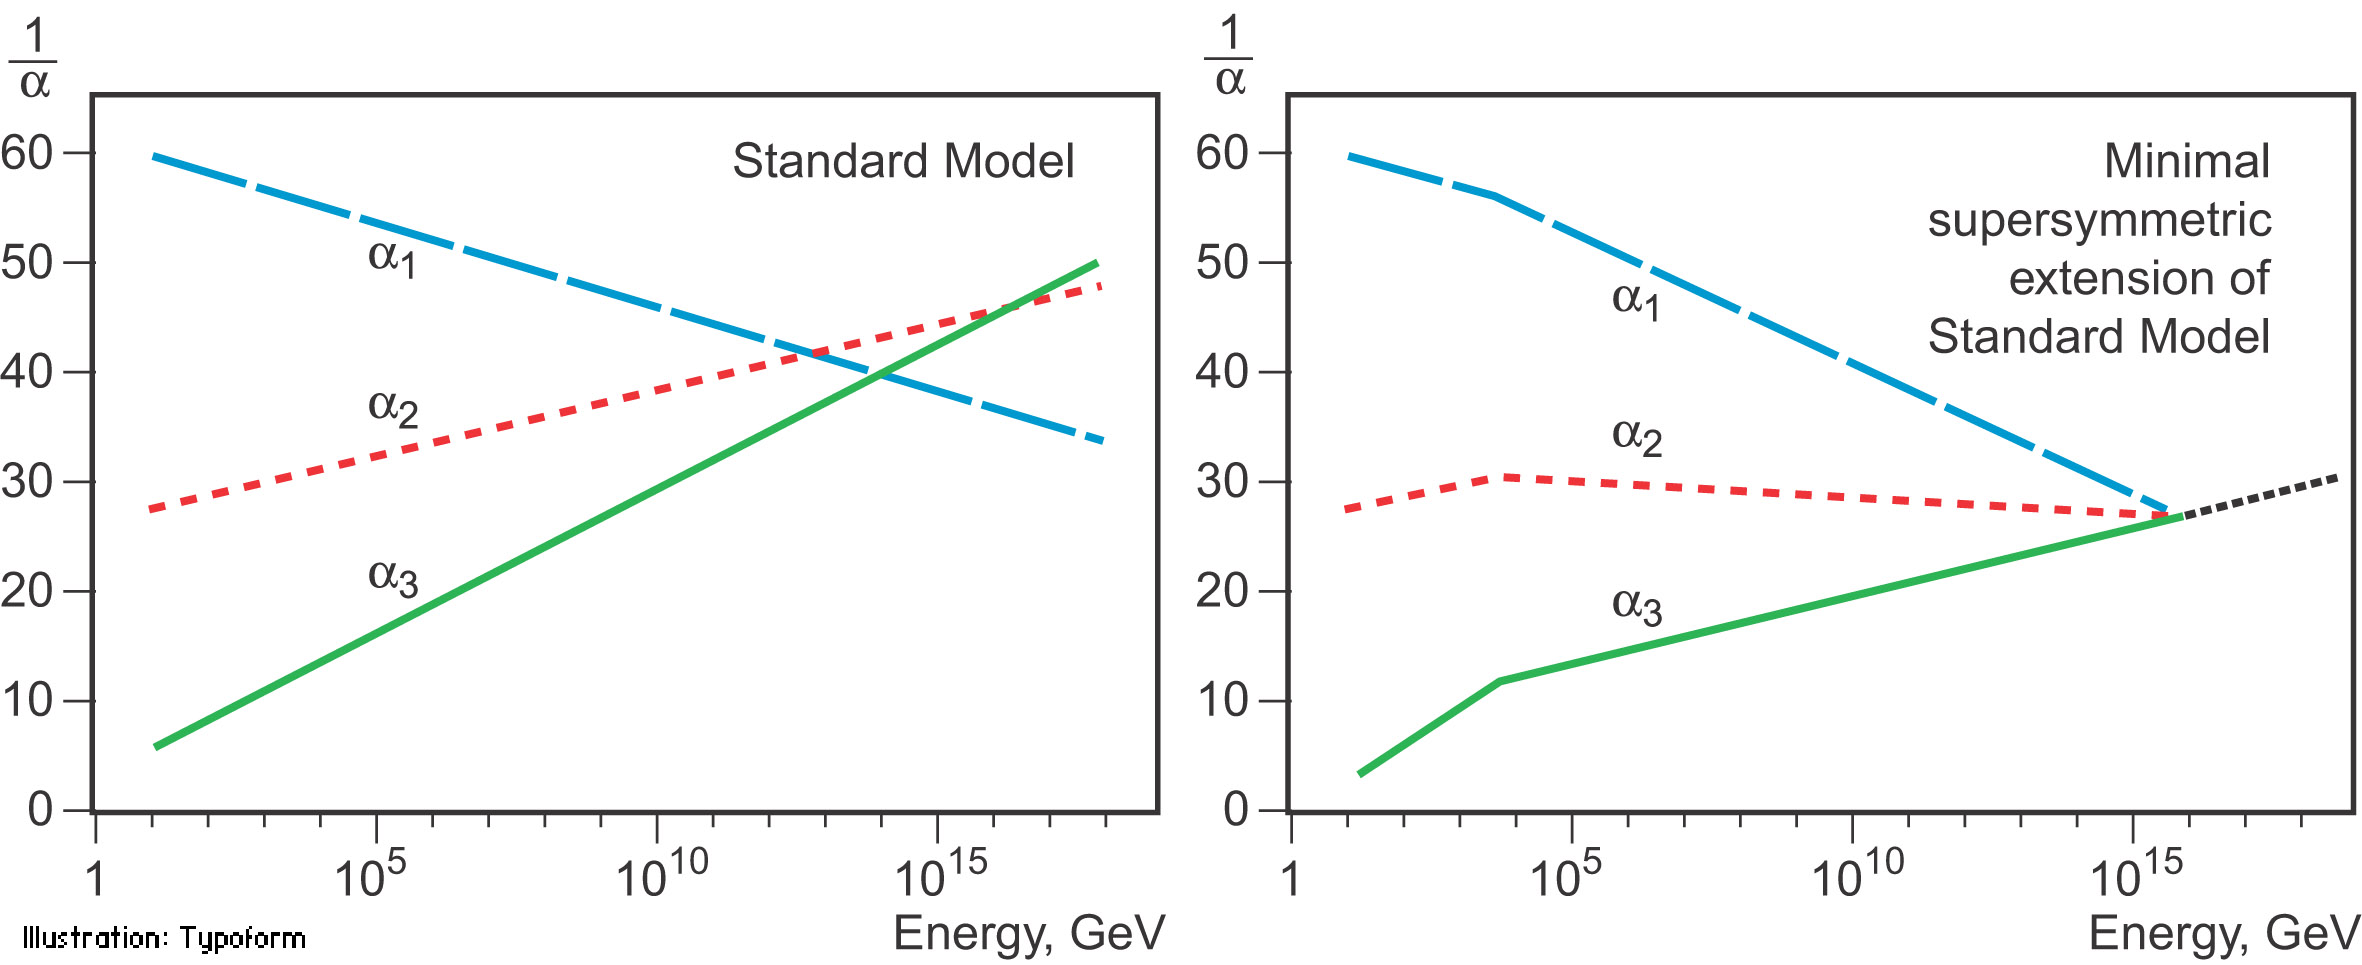
\includegraphics[scale=0.7]{figs/coupling_constants.jpg}
\caption{Running coupling constants as a function of the energy scale, for the SM (left) and in the context of supersymmetry (right)~\cite{CouplingConstants} \label{fig:constants}}
\end{center}
\end{figure}
 
\begin{itemize} 
\item The number of fermion families. As mentioned earlier, the number of fermion families is not an observable, but rather an input for the theory. More generations could in principle be accommodated as part of the SM particle content. 
\item The gauge hierarchy problem. This is intrinsically related to the mass of the Higgs boson. Apart from the fact that it is not predicted by the theory, it requires fine-tuning in order not to diverge, leading to the enlargement of the EW scale. Also, it is very small compared to the gravity scale, given by the Planck mass: $M_{Pl} = \sqrt{\hbar c/G_N} = 1.2 \times 10^{19} \GeV$, which is not fully understood. 
\item Inclusion of gravity. The SM fails to include gravity as one of the interactions, as there is no quantum theory for it. 
\item Neutrino masses. As it was already mentioned before, neutrinos are massless within the SM model. Nevertheless, experimental observations such as the oscillations of solar neutrinos\red{~\cite{SolarNeutrinos}} prove this prediction wrong. Thus, a Beyond the SM (BSM) mechanism to give neutrinos mass is required. There are several proposals for this, such as the seesaw mechanism or the Majorana theory\red{~\cite{Seesaw}}. 
\item Charge quantisation. The fact that the electron charge and the proton charge are of the same magnitude but opposite sign has no explanation in the SM. 
%\item \red{Strong CP problem}
\item Fermion masses and mixing angles. Similarly to what happened with the number of fermion families, these quantities are not predicted by the SM. Moreover, the mass of the top quark, much bigger than the other quark masses, is an intriguing fact not explained by this theory. 
\item The magnetic dipole moment of the muon, whose experimental measurement\red{~\cite{MuonDM}} deviates more than 3$\sigma$ from the SM predictions. 
\end{itemize}

In addition to this, several results provided by the LHCb collaboration \red{refs} on flavour anomalies and lepton flavour universality studies contribute to the motivation of the search for BSM physics. 

Several theories have been proposed to cope with the SM problems, that make this model look more like an effective low energy theory than a model itself. Among these, Supersymmetry and Minimal Flavour Violation (MFV) are of special importance and will be discussed in the following chapters. However, there are other alternatives, some of which are briefly discussed below.

\begin{itemize}
\item \textbf{Majorana neutrinos}: in the SM, neutrinos are supposed to be massless \textit{Dirac} particles. However it's been suggested that they are instead its own antiparticle, \textit{Majorana neutrinos}. Within this theory, they are allowed to acquire mass. Several experiments search for a neutrinoless double beta decay that would prove this~\cite{KamLAND-Zen:2016pfg},~\cite{GERDA}.
\item \textbf{Axions}: axions are hypothetical particles that compose DM, including the Peccei-Quinn mechanism~\cite{Axions1} to solve the \red{strong CP problem}~\cite{StrongCP}. They would have been massively produced soon after the Big Bang. The couplings and masses axions can cover several orders of magnitudes. %%%https://arxiv.org/pdf/1712.03018.pdf %% http://iaxo.web.cern.ch/content/physics
\item \textbf{Two Higgs Doublet Models (THDM)}: in this scenario, there are two Higgs fields populating the vacuum instead of one. %% https://arxiv.org/pdf/1106.0034.pdf
\begin{equation}
\left \langle \phi_a \right \rangle_0 = \binom{0}{\frac{v_1}{\sqrt{2}}}, \ \left \langle \phi_b \right \rangle_0 = \binom{0}{\frac{v_2}{\sqrt{2}}}
\end{equation}
Where $v_2$ and $v_2$ follow the relation:
\begin{equation}
v \equiv (v_1^2 + v_2^2)^{1/2}
\end{equation}
The ratio between these two VEVs, $\tan{\beta} \equiv \frac{v_2}{v_1}$ is the most important parameter in this model. It describes the diagonalization of the mass-squared matrices of the charged scalars and of the pseudoscalars, resulting in 4 fields
\begin{equation}
\begin{split}
& \phi_1 = \sin{\beta}\phi_b + \cos{\beta}\phi_a \ \phi_2 = -\sin{\beta}\phi_a + \cos{\beta}\phi_b \\
& \left \langle \phi_1 \right \rangle_0 = \binom{0}{\frac{v_{SM}}{\sqrt{2}}}, \ \left \langle \phi_2 \right \rangle_0 = \binom{0}{0}
\end{split}
\end{equation}
The spontaneous symmetry breaking leads in this case to 5 physical Higgs particles: two neutral scalars linear combinations of $Re(\phi_1^0)$ and $Re(\phi_1^0)$, $H^0$ and $h^0$; a neutral pseudoscalar, $A^0 \propto Im(\phi_2^0)$ and two charged scalars $H^\pm = \phi_2^\pm$.  
\item \textbf{Models with extra dimensions}: models with extra dimensions (apart from the usual 4 from the observed spacetime) are motivated by the attempts made to unify electromagnetism and gravity within the Kaluza-Klein theory~\cite{Kaluza},~\cite{Klein}. There are several proposals, such as \textit{string theory} or the \textit{Randall-Sundrum model}~\cite{RS}, that gives explanation to hierarchy using 5 dimensions and predicts the existence of the \textit{graviton}. 
\item \textbf{SM with fourth generation (SM4)}: adding a fourth generation of fermions requires the corresponding neutrino to be heavy, $m_{\nu_4} > M_Z/2$, to match the current experimental constraints~\cite{Lenz:2013iha}.   %%https://cds.cern.ch/record/1635712/files/910275.pdf
\item \textbf{Little Higgs Models}: in these models, the Higgs is realised as a light pseudo-Nambu Goldstone boson of a broken global symmetry. They attempt to solve the gauge hierarchy problem. The minimal version of such models include 4 new heavy vector bosons, ($W'^{\pm}$, $Z'$, $B'$), coupled to SM fermions, mixed with the SM $W^{\pm}$ and $Z$;  light Higgs doublet(s), with possibility of extra light scalar multiplets; heavy Higgs multiplets, coupled to Higgs/Goldstone pairs, decoupled from fermions, mixed with light Higgses, and heavy up-type quark(s), $t'$. An example spectrum can be seen in \ref{fig:lhm}. Updated constraints in this model can be found in~\cite{LHM}.
   %%https://arxiv.org/pdf/1703.10190.pdf %%http://www.desy.de/~reuter/downloads/lhm.pdf
\begin{figure} [htb!]
\begin{center}
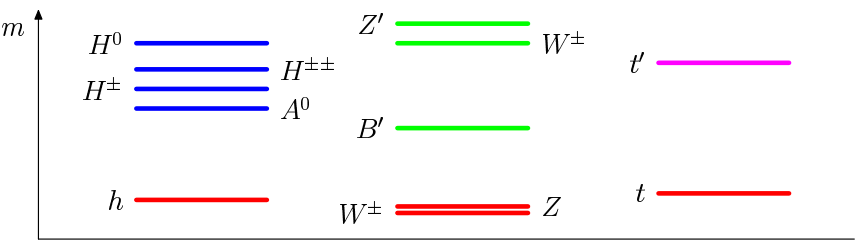
\includegraphics[scale=0.7]{figs/lhm.png}
\caption{Example spectrum for LHM \red{ref?} \label{fig:lhm}}
\end{center}
\end{figure}
\end{itemize}

 % Max 5 pages

%% Theory
%\blankpage
%\input{chapters/Theory}

%% The LHCb experiment
%\blankpage
%\input{chapters/LHCb-experiment} 



%% Analysis
%\chapter{Conclusions}
\label{sec:Conclusions}


\cleardoublepage
%\phantomsection
%\addcontentsline{toc}{section}{References}
%\bibliographystyle{chapters/LHCbStyle}
%\bibliography{chapters/References}

\addcontentsline{toc}{section}{References}
\setboolean{inbibliography}{true}
\bibliographystyle{LHCb}
\bibliography{main,LHCb-PAPER}


\end{document}
